\documentclass[a4paper]{article}
\usepackage{color}              %Farben, f.r \definecolor{}
\usepackage{amssymb}            %Mathematische Symbole
\usepackage{amsthm}             %Besseres \newtheorem
\usepackage{amsmath}           %Mathematische Umgebungen
\usepackage{mathtools}          %\xRightarrow, etc
\usepackage{mathrsfs}           %enthaelt \mathscr
\usepackage{graphicx}
\usepackage{enumerate}          % in-place numerations def.
\usepackage{fullpage}

\usepackage{array}
%\usepackage{multicol}
%\usepackage[notref,notcite]{showkeys}
%\usepackage{algorithm,algorithmic}
\usepackage{color}

\usepackage{graphicx}
\usepackage{xypic}
\entrymodifiers={+!!<0pt,\fontdimen22\textfont2>}
\usepackage[all]{xy}
\usepackage{tikz}

\newtheoremstyle{myremark} % name
    {7pt}                    % Space above
    {7pt}                    % Space below
    {}  	                 % Body font
    {}                           % Indent amount
    {\bf}       	         % Theorem head font
    {.}                          % Punctuation after theorem head
    {.5em}                       % Space after theorem head
    {}  % Theorem head spec (can be left empty, meaning ‘normal’)

\theoremstyle{plain}
\newtheorem{lemma}{Lemma}
\newtheorem{theorem}[lemma]{Theorem}
\newtheorem{fact}[lemma]{Fact}
\newtheorem{definition}[lemma]{Definition}
\newtheorem{corollary}[lemma]{Corollary}
\newtheorem{proposition}[lemma]{Proposition}
\newtheorem{conjecture}[lemma]{Conjecture}
\newtheorem{observation}[lemma]{Observation}
\newtheorem{problem}[lemma]{Problem}
\newtheorem{notation}[lemma]{Notation}
\newtheorem*{claim}{Claim}

\theoremstyle{myremark}
\newtheorem{remark}[lemma]{Remark}
\newtheorem{example}[lemma]{Example}

%%%%%% EDIT HERE: %%%%%%%%%%%
\newcommand{\LECTURENUMBER}{6}
\newcommand{\LECTURETITLE}{Lists, triangulation and the art gallery problem}
\newcommand{\LECTURESCRIBE}{Kristoffer Nielsen}

%% Dokument Beginn %%%%%%%%%%%%%%%%%%%%%%%%%%%%%%%%%%%%%%%%%%%%%%%%%%%%%%%%
\begin{document}
\thispagestyle{empty}

\begin{center}
	{\Large\bf Graph coloring}\\
	{\bf Lecture notes, vol. \LECTURENUMBER, \LECTURETITLE}\\
\end{center}
Lecturer: Michal Adamaszek \hfill Scribe: \LECTURESCRIBE
\begin{center}
\line(1,0){450}
\end{center}

%%%%%%% EDIT ALSO BELOW: %%%%%%%%%%%%%%%%

\begin{theorem}[5-color theorem]
If $G$ is planar then $\chi(G) \leq 5$.
\end{theorem}
\begin{proof}
Later: "Proof from the book" (Aigner, Zeigler).
\end{proof}

List coloring, examples:
\begin{itemize}
\item[1]A graph $G(V,E)$ with
	\begin{itemize}
	\item V = courses
	\item E = conflicts (student in both courses)
	\end{itemize}
	can be subject to a list-coloring should there restrictions to for instance  the choices of days that a course can be held at. 
\item[2]Soduku $\equiv$ coloring of $9\times 9$ grid with restrictions in the form of already given numbers.
\end{itemize}

As a definition:
\begin{definition}
Let $G$ be any graph, for every vertex $x\in V(G)$ we have a set of colors $L(x)$ ( of colors available to $x$).

A $L$-coloring of $G$ is a coloring $c:V(G)\rightarrow \underset{x}{\bigcup} L(x)$ such that $c(x)\in L(x)$ for all $x$. 

The list-chromatic number $\chi_{\ell}(G)$ is the smallest $k$ s.t. $G$ has a $L$-coloring for any choice of list satisfying $|L(x)|\geq k$. 

$G$ is $k$-list-colorable ($k$-choosable) when $\chi_{\ell}(G)\leq k$.
\end{definition}

\begin{example}
Here are some various examples and facts:

\begin{itemize}
\item $L(x)=\{1,\ldots,k\}$ for all $x\in V(G)$ then $L$-coloring $\equiv$ $k$-coloring in the normal sense
\item $\chi(G)\leq \chi_{\ell}(G)$
\item Example with $\chi(G) < \chi_{\ell}(G)$:
\begin{center}
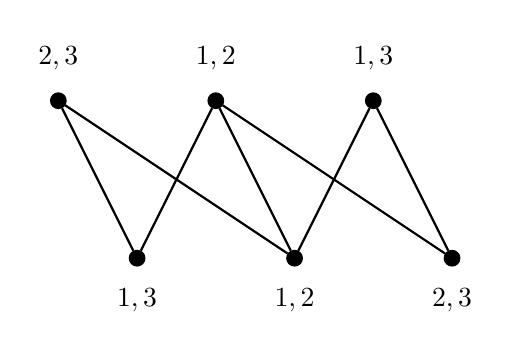
\begin{tikzpicture}[
every node/.style={circle,inner sep=2pt,fill,draw}
]
\node[label={[label distance=1pt]90:$2,3$}] (A) at (-2,1) {};
\node[label={[label distance=1pt]90:$1,2$}] (B) at (0,1) {};
\node[label={[label distance=1pt]90:$1,3$}] (C) at (2,1) {};

\node[label={[label distance=1pt]270:$1,3$}] (D) at (-1,-1) {};
\node[label={[label distance=1pt]270:$1,2$}] (E) at (1,-1) {};
\node[label={[label distance=1pt]270:$2,3$}] (F) at (3,-1) {};

\draw[thick] (A) -- (D);
\draw[thick] (A) -- (E) ;

\draw[thick] (B) -- (D);
\draw[thick] (B) -- (F);
\draw[thick] (B) -- (E);

\draw[thick] (C) -- (E);
\draw[thick] (C) -- (F);

\end{tikzpicture}
\end{center}
For each $x$, $|L(x)|=2$. But for these list there are no $L$-coloring. Therefore $\chi_{\ell}(G)\geq 3$, while $\chi(G)=2$ since the graph is bipartite.
\item $\chi_{\ell}(G)\leq \Delta G+1$, same proof as the non-list chromatic number.
\item Brooks Theorem holds.
\end{itemize}
\end{example}

\textbf{Question:} Can we construct $G$ with small $\chi(G)$ and large $\chi_{\ell}(G)$?

\begin{proposition}
For every $k\geq 2$ there exist a graph with $\chi(G)=2$ and $\chi_{\ell}(G)>k$
\end{proposition}

\begin{proof}
Take $A=B=\binom{\{1,\ldots,2k-1\}}{k}$, (the set of all $k$-subsets of $\{1,\ldots,2k-1\}$).

Let $G=K_{A,B}$ be the complete bipartite graph with parts $A$ and $B$.
\begin{example}
Take $k=3, |A|=|B|=\binom{5}{3}=10$

That is $A$ and $B$ will consist of 10 vertices each with a list of three numbers made of the various permutations of $[1,2,3,4,5]$ and every vertex in $A$ is connected to every vertex in $B$. So $|V|=20, |E|=100$.
\end{example}

(\textit{proof} cont.)
For $X \in A$ or $X \in B$ set $L(X)=X$ and note $|L(X)|=k.$
We claim that $K_{A,B}$ has no $L$-coloring.

Suppose $c$ is an $L$-coloring. Then $c(A)\subseteq \{1,\ldots,2k-1\}$, $|c(A)|\geq k$. $\leftarrow$ will be true, or otherwise $|c(A)|\leq k-1$ and then there is a $X\subseteq\{1,\ldots,2k-1\}$ such that $|X|=k$ and $X\cap c(A)=\emptyset$. Then $X$ cannot be colored with a color from $L(X)$.

Similar for $B$, that is  $c(B)\subseteq \{1,\ldots,2k-1\}$, $|c(B)|\geq k$.

It follows  that $c(A)\cap c(B)\neq \emptyset$ so two vertices on opposite sides have the same color. That means $\chi_{\ell}(K_{A,B})\geq k+1$, but $\chi(K_{A,B})=2$.
\end{proof}

\begin{theorem}
(Thomassen 1994)

Every planar graph satisfies $\chi_{\ell}(G)\leq 5$. (It is 5-list-colorable).  
\end{theorem}
\begin{remark}
This is stronger than the 5-color theorem, because $\chi(G)\leq \chi_{\ell}(G)$.
\end{remark}

\begin{definition}
An embedding of a planar graph $G$ is called:
\begin{itemize}
\item A triangulation if every face is a triangle (also the unbounded one)
\item A near-triangulation if every bounded face is a triangle and the unbounded one is a cycle.
\end{itemize}
\end{definition}

\begin{example}
Various examples of Definition 8.
\begin{center}
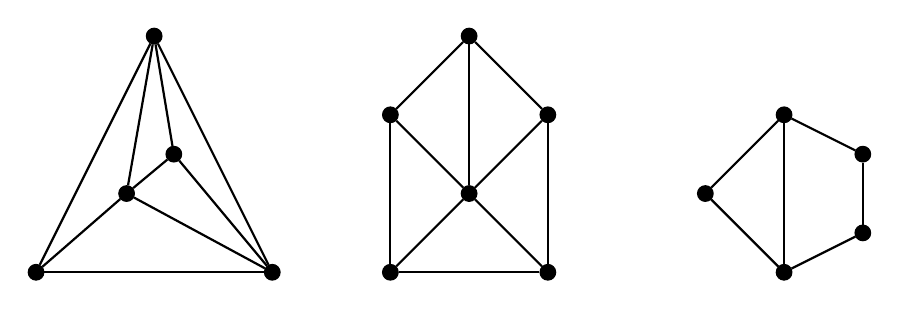
\begin{tikzpicture}[
every node/.style={circle,inner sep=2pt,fill,draw}
]
\node (a) at (-5,2) {};
\node (b) at (-5.35,0) {};
\node (c) at (-4.75,0.5) {};
\node (d) at (-6.5,-1) {};
\node (e) at (-3.5,-1) {};

\draw[thick] (a) -- (b);
\draw[thick] (a) -- (c) ;
\draw[thick] (a) -- (d);
\draw[thick] (a) -- (e);
\draw[thick] (b) -- (c);
\draw[thick] (b) -- (d);
\draw[thick] (b) -- (e);
\draw[thick] (d) -- (e);
\draw[thick] (c) -- (e);

\node (f) at (-2,-1) {};
\node (g) at (-2,1) {};
\node (h) at (-1,0) {};
\node (i) at (-1,2) {};
\node (j) at (0,-1) {};
\node (k) at (0,1) {};

\draw[thick] (f) -- (g);
\draw[thick] (g) -- (i);
\draw[thick] (i) -- (k);
\draw[thick] (j) -- (k);
\draw[thick] (j) -- (f);
\draw[thick] (h) -- (f);
\draw[thick] (h) -- (g);
\draw[thick] (h) -- (i);
\draw[thick] (h) -- (k);
\draw[thick] (h) -- (j);

\node (l) at (2,0) {};
\node (m) at (3,1) {};
\node (n) at (3,-1) {};
\node (o) at (4,0.5) {};
\node (p) at (4,-0.5) {};

\draw[thick] (l) -- (m);
\draw[thick] (m) -- (o);
\draw[thick] (o) -- (p);
\draw[thick] (p) -- (n);
\draw[thick] (n) -- (l);
\draw[thick] (n) -- (m);

\end{tikzpicture}
\end{center}
From left to right: A triangulation, a near triangulation and the final picture is neither.
\end{example}

\begin{remark}
Every embedding can be extended to a triangulation on the same vertex set. (By only adding edges)
\end{remark}
\begin{proof}
Add diagonals as needed. It also work for the unbounded face.
\end{proof} 

In other words:
For any planar $G$ there is a triangulation $H$ such that
\begin{align*}
V(G)=V(H), \ E(G)\subseteq E(H).
\end{align*} 
In particular
\begin{align*}
\chi(G) &\leq \chi(H)
\\
\chi_{\ell}(G) &\leq \chi_{\ell}(H)
\end{align*}

\begin{proposition}
Suppose $G$ is near-triangular with outer cycle $\mathbb{O}=x_1,\ldots,x_k$ and assume the following exist:
\begin{itemize}
\item $L(x_1)=\{a\}$, $L(x_2)=\{b\}$, $a\neq b$
\item $|L(x_i)|\geq 3$ for all $i=3,\ldots,k-1$
\item $|L(y)|\geq 5$ for all $y\notin \mathbb{O}$.
\end{itemize}
Then $G$ is L-colorable.
\end{proposition}

\begin{remark}
This proposition implies Thomassens theorem as follows:

Take $H$, any planar graph, with lists $L$ and $|L(x)| \geq 5$. Extend $H$ to a triangulation $H\subseteq G$ (in particular, $G$ is a near-triangulation). Choose any $x_1,x_2$ on the outer face. Restrict $L(x_1)$ and $L(x_2)$ to one element and voila! $\rightarrow$ the proposition applies to $G$. 

$L$-coloring of $G$ gives an $L$-coloring for $H$.
\end{remark}

\begin{proof}
Proof of proposition 11:

\begin{itemize}
\item $|V(G)|=3$: 
\begin{center}
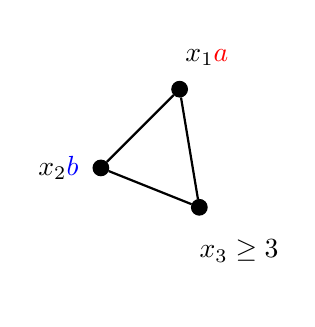
\begin{tikzpicture}[
every node/.style={circle,inner sep=2pt,fill,draw}
]
\node[label={[label distance=1pt]60:$x_1 {\color{red}a}$}] (A) at (1,1) {};
\node[label={[label distance=1pt]180:$x_2 {\color{blue}b}$}] (B) at (0,0) {};
\node[label={[label distance=1pt]300:$x_3 \geq 3$}] (C) at (1.25,-0.5) {};


\draw[thick] (A) -- (B);
\draw[thick] (A) -- (C) ;
\draw[thick] (B) -- (C);

\end{tikzpicture}
\end{center}
Then we will have a spare color for $x_3$.
\end{itemize}

\underline{Case 1}:

There is an edge $x_k x_j$, $j=2,\ldots,k-2$
\begin{center}
\includegraphics[scale=0.25]{Case1}
\end{center}
\begin{itemize}
\item[•]$G_1=$ graph bounded by $x_1x_2\ldots x_jx_k \rightarrow$ $L$-color $G_1$ by induction.
\item[•] $G_2=$ graph bounded by $x_kx_j\ldots x_{k-1} \rightarrow $ $L$-color $G_2$ by induction.
\item[•] $\rightarrow$ L-coloring of $G$. Note that after coloring $G_1$ some colors are not available for certain vertices of $G_2$, but there is enough left just to use the induction hypothesis for $G_2$.
\end{itemize}

\underline{Case 2}:

There are no edge $x_k x_j$, $j=2,\ldots,k-2$.
\begin{itemize}
\item Around $x_k$ we must have a sequence of triangles, since the interior is triangulated.
\item Let $N(X_k)=\{x_1,x_{k-1},y_1,\ldots,y_{\ell}\}$
\item Pick $c,d \in L(X_k)$, $c\neq d$, $c,d \neq a$.
\item Set $G'=G-x_k$ and note that $G' $ is a near-triangulation. 
\end{itemize}
\begin{center}
\includegraphics[scale=0.125]{Case2}
\end{center}
Consider the list:
\begin{align*}
L'(y_i)=L(y_i)\backslash \{c,d\} \ , \ L'(x)=L(x) \ \text{for any other} \ x \in G'
\end{align*}
$\leadsto$ There is a L'-coloring of $G'$ by induction.
\begin{align*}
c(y_i)\notin \{c,d\} \ , \ c(x_1) \notin \{c,d\}
\end{align*}
$\leadsto$ color $x_k$ with either $c$ or $d$ depending on $c(x_{k-1})$.
\end{proof}

\begin{remark}
There are planar not-4-list-colorable graphs. (Voigt '93 example with $\approx$ 300 vertices).
\end{remark}
\begin{remark}
Did not use Euler, upper/lower bounds. Only geometric properties.
\end{remark}
\subsubsection*{Application:
\underline{The art gallery problem}}

Suppose $P$ is a polygon in $\mathbb{R}^2$ with $n$ vertices.

\begin{example}
:
\begin{center}
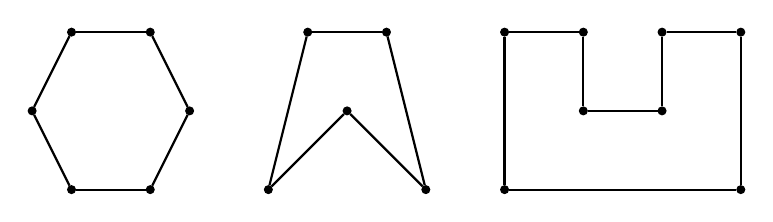
\begin{tikzpicture}[
every node/.style={circle,inner sep=1pt,fill,draw}
]
\node (a) at (-4,0) {};
\node (b) at (-3.5,1) {};
\node (c) at (-3.5,-1) {};
\node (d) at (-2.5,1) {};
\node (e) at (-2.5,-1) {};
\node (f) at (-2,0) {};

\draw[thick] (a) -- (b);
\draw[thick] (a) -- (c) ;
\draw[thick] (b) -- (d);
\draw[thick] (d) -- (f);
\draw[thick] (e) -- (f);
\draw[thick] (e) -- (c);

\node (g) at (-1,-1) {};
\node (h) at (-0.5,1) {};
\node (i) at (0,0) {};
\node (j) at (0.5,1) {};
\node (k) at (1,-1) {};

\draw[thick] (h) -- (g);
\draw[thick] (g) -- (i);
\draw[thick] (h) -- (j);
\draw[thick] (j) -- (k);
\draw[thick] (k) -- (i);

\node (l) at (2,-1) {};
\node (m) at (2,1) {};
\node (o) at (3,1) {};
\node (p) at (3,0) {};
\node (q) at (4,0) {};
\node (r) at (4,1) {};
\node (s) at (5,1) {};
\node (t) at (5,-1) {};

\draw[thick] (l) -- (m);
\draw[thick] (m) -- (o);
\draw[thick] (o) -- (p);
\draw[thick] (p) -- (q);
\draw[thick] (q) -- (r);
\draw[thick] (r) -- (s);
\draw[thick] (s) -- (t);
\draw[thick] (t) -- (l);


\end{tikzpicture}
\end{center}

\end{example}

We assume the bounded region is the floor plan af an art gallery.
\begin{quote}
How many guards are needed to guard each point in sight?
\end{quote}

\begin{problem}
\begin{itemize}
\item Find a gallery with 6 vertices requiring $\geq 2$ guards.
\item Find a gallery with as few vertices as possible requiring $\geq k$ guards.
\end{itemize}
\end{problem}

\begin{observation}
There are $n$-vertex galleries requiring at least $\left \lfloor \frac{n}{3} \right \rfloor$ guards.
\end{observation}
\begin{center}
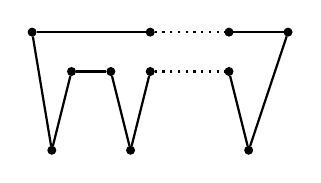
\begin{tikzpicture}[
every node/.style={circle,inner sep=1pt,fill,draw}
]
\node (a) at (-3.5,1.5) {};
\node (b) at (-3.25,0) {};
\node (c) at (-3,1) {};
\node (d) at (-2.5,1) {};
\node (e) at (-2.25,0) {};
\node (f) at (-2,1) {};
\node (g) at (-1,1) {};
\node (h) at (-0.75,0) {};
\node (i) at (-0.25,1.5) {};
\node (f') at (-2,1.5) {};
\node (g') at (-1,1.5) {};

\draw[thick] (a) -- (b);
\draw[thick] (b) -- (c) ;
\draw[thick] (c) -- (d);
\draw[thick] (d) -- (e);
\draw[thick] (e) -- (f);
\draw[dotted, thick] (f) -- (g);
\draw[thick] (g) -- (h);
\draw[thick] (h) -- (i);
\draw[dotted, thick] (f') -- (g');
\draw[thick] (i) -- (g');
\draw[thick] (a) -- (f');

\end{tikzpicture}
\end{center}

\begin{theorem}
Rephrasing the art gallery problem:

Every n-vertex gallery can be guarded by $\left \lfloor \frac{n}{3} \right \rfloor$ guards. ($\approx$ 70's Chvatal).
\end{theorem}

\begin{definition}
A planar embedding is called a \emph{polygon triangulation} if it is a near-triangulation and all vertices lie on the outer cycle.
\end{definition}

\begin{example}
"Polygon triangulated by diagonals"
\begin{center}
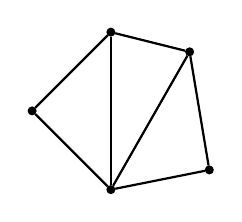
\begin{tikzpicture}[
every node/.style={circle,inner sep=1pt,fill,draw}
]
\node (a) at (-1,0) {};
\node (b) at (0,1) {};
\node (c) at (0,-1) {};
\node (d) at (1,0.75) {};
\node (e) at (1.25,-0.75) {};

\draw[thick] (a) -- (b);
\draw[thick] (a) -- (c);
\draw[thick] (c) -- (b);
\draw[thick] (d) -- (c);
\draw[thick] (b) -- (d);
\draw[thick] (c) -- (e);
\draw[thick] (d) -- (e);

\end{tikzpicture}
\end{center}
\end{example}

\begin{observation}
A triangulated polygon with n vertices has $2n-3$ edges, $n$ on the outer cycle and $n-3$ diagonals.
\end{observation}

\begin{observation}
Every triangulated polygon have a vertex of degree 2.
\end{observation}
\begin{proof}
The shortest diagonal cuts off such a vertex.
\end{proof}

\begin{observation}
Every triangulated polygon is 3-colorable.
\end{observation}
\begin{proof}
Take $v$ to be a vertex of degree 2. $G-v$ is a triangulated polygon. Color $G-v$ with 3 colors, the neighbours of $v$ will use 2 colors. Color $v$ with the spare color.
\end{proof}

\begin{proof}
Proof of Theorem 18:

\begin{itemize}
\item Let $G$ be planar polygon with $n$ vertices.
\item First triangulate using diagonals (Exercise: show that this is always possible).
\item The resulting triangular polygon is 3-colorable. 
\item Some color class will have $\leq \left \lfloor \frac{n}{3} \right \rfloor$ elements
\item Place guards at the vertices of that color.
\end{itemize}
\end{proof}
%%%%%%%%%%%%%%%%%%%%%%%%%%%%%%%%%%%%%%%%

\end{document}




